\chapter{Ciclo 1}
  
  Este capítulo descreve o planejamento realizado e os resultados obtidos com a execução do primeiro ciclo da pesquisa-ação.
  
  \section{Planejamento}
  
      Após a realização do diagnóstico, era necessário um esforço inicial de configuração do \textit{framework} para a 
      adequação do PHPUnit ao CodeIgniter. Além disso, era necessário estabelecer a estrutura do \textit{framework},
      sua arquitetura de funcionamento. Portanto, ficaram definidas como escopo do primeiro ciclo as seguintes atividades:
      
      \begin{itemize}
    
    \item Configurar o CodeIgniter para receber o PHPUnit;
    
    \item Estabelecer arquitetura de funcionamento do \textit{framework}.
    
      \end{itemize}
      
      
      \subsection{Planejamento da avaliação}
      
      Como este ciclo não agregou muito valor para a atividade de testes dos desenvolvedores do SiGA,
      embora imprescindível para o \textit{framework}, o mesmo teve uma forma de avaliação diferente
      dos outros ciclos (não avaliado pelo questionário proposto) por não envolver diretamente os desenvolvedores e se
      tratar de conteúdo mais técnico inerente à equipe de desenvolvimento do \textit{framework}. Visto isso, ficou proposta
      a seguinte estrutura de avaliação para as atividades realizadas neste ciclo:
      
      \begin{itemize}
      
        \item Para a atividade de configuração do CodeIgniter para o uso do PHPUnit:
      
        \begin{enumerate}
          
          \item Testar as configurações propostas em um projeto vazio do CodeIgniter versão 2.x;
          
          \item Testar as configurações propostas no SiGA;
          
        \end{enumerate}
          
        \item Para a atividade de estabelecimento da arquitetura de funcionamento do \textit{framework}:
        
        \begin{enumerate}
    
          \item Validar a arquitetura proposta implementando os comandos \textit{\textbf{init}} e \textit{\textbf{help}};
              
              \subitem Se atentar aos seguintes itens indispensáveis:
            \begin{itemize}
              \item É fácil de se criar um novo comando?
              \item É possível criar um comando com parâmetros diferentes?
              \item É possível ter parâmetros opcionais nos comandos?
              \item É possível tratar cada comando individualmente e executá-los em conjunto?
            \end{itemize}
          
          \item Testar o comando \textit{\textbf{init}} em um projeto vazio do CodeIgniter versão 2.x;
          
          \item Testar o comando \textit{\textbf{init}} no SiGA;
    
          \item Testar o comando \textit{\textbf{help}};
        \end{enumerate}
      
      \end{itemize}
  
  \section{Execução do ciclo}
  
      Esta seção apresenta detalhes relacionados à execução do ciclo 1.
      
      \subsection{Arquitetura do \textit{Ignitest}}
      
	  Para o contexto proposto, onde existirão vários comandos que possuem comportamentos únicos e bem definidos que serão
	  invocados pela linha de comando, a arquitetura definida se baseia no padrão de projeto \textit{Command} \cite{gamma}
	  com a adição de classes \textit{experts} (padrão GRASP) de metadados para cada comando, como pode ser visto na
	  figura \ref{ignitest-architecture}.
	   
	  As classes filhas da classe \textit{Command} representam um comando específico do \textit{framework} que possui sua 
	  própria implementação de execução. Cada comando possui uma classe de metadados associada a ele para descrever suas
	  informações, onde essa classe deve herdar da classe \textit{Metadata}. Os comandos informados pela linha de comando (CLI)
	  são interpretados pela classe \textit{CommandChecker}, que verifica os comandos informados, cria as instâncias respectivas
	  e adiciona os comandos na fila de execução. Os comandos disponíveis no \textit{framework} devem ser registrados na classe
	  \textit{AvailableCommand} para que seja possível a classe \textit{CommandChecker} identificar os comandos informados.
	  
	  \vfill
	  \pagebreak
	  \begin{figure}[!htb]
	    \centering
	    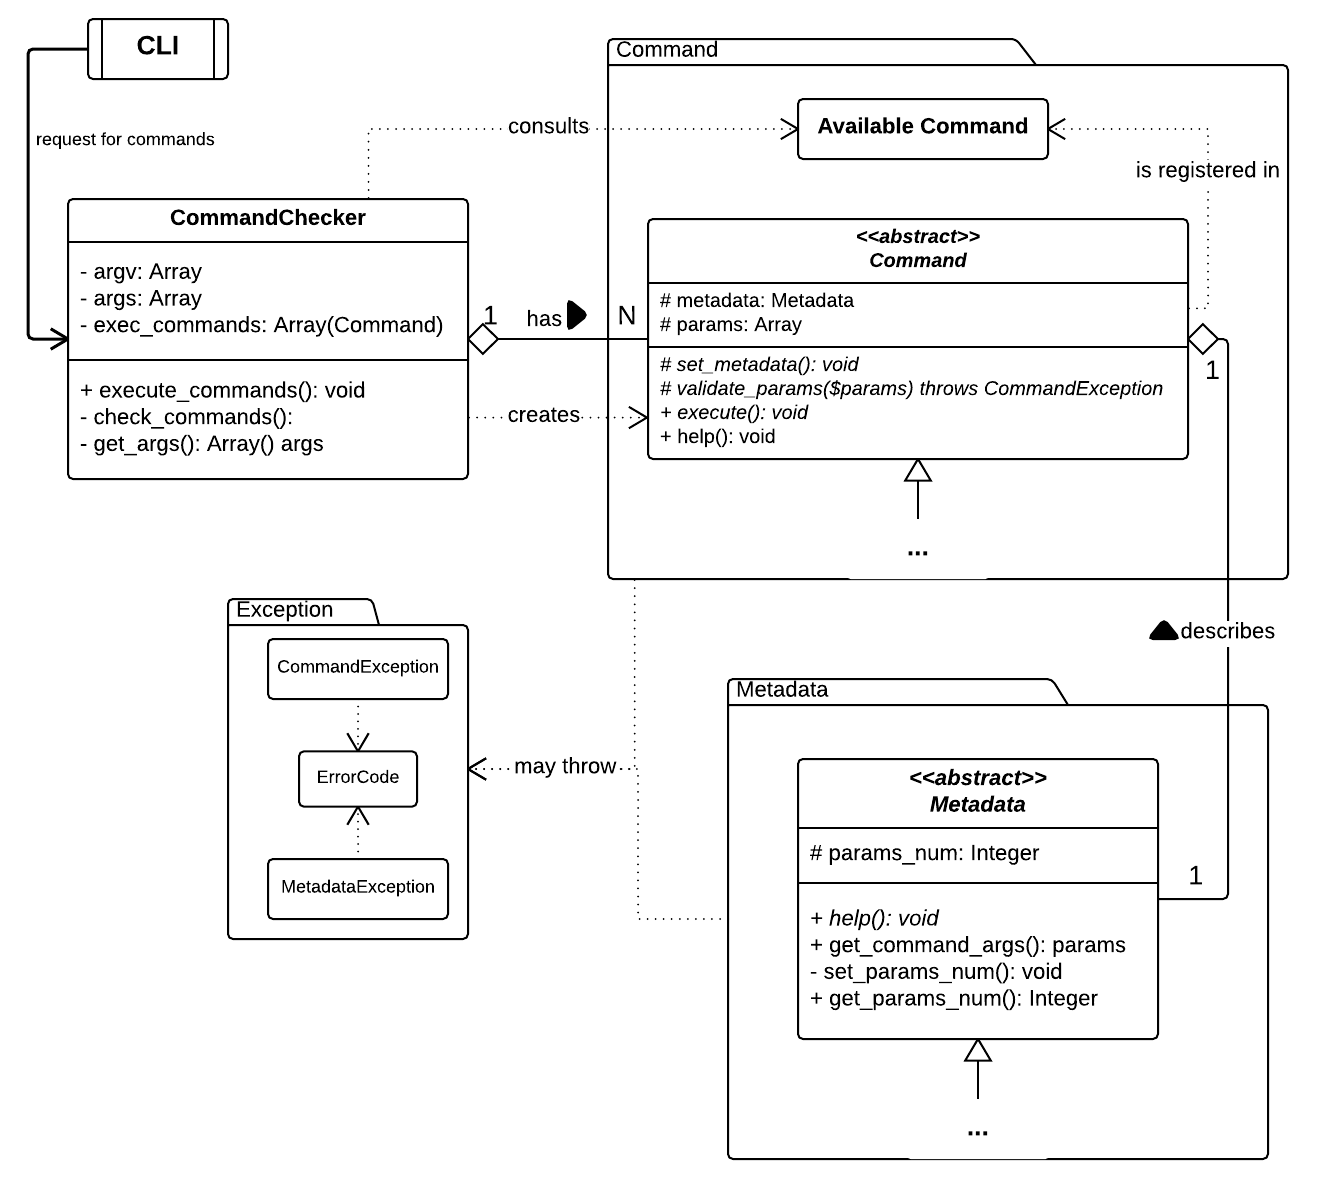
\includegraphics[scale=0.35]{figuras/ignitest-architecture.png}
	    \caption{Arquitetura do \textit{framework} proposto.}
	    \label{ignitest-architecture}
	  \end{figure}
      
      \subsection{Configurações}
	  
	  Para que o PHPUnit funcione no CodeIgniter, descobriu-se que era preciso definir um \textit{hook}\footnotemark
	  no projeto para mostrar os resultados do PHPUnit caso o ambiente fosse de teste, pois ao executar o PHPUnit nenhum
	  resultado era disponibizado na tela. Foi preciso seguir os seguintes passos para resolver esse problema:
	  \footnotetext{CodeIgniter Hooks. Disponível em \url{http://www.codeigniter.com/userguide2/general/hooks.html}. Acesso em 20/06/2016.}
	  
	  \begin{itemize}
	  
	   \item Habilitar o uso de \textit{hooks} no CodeIgniter no arquivo '\textbf{application/config/config.php}':
	      
	      \begin{verbatim}
		$config['enable_hooks'] = TRUE;
	      \end{verbatim}
	      
	   \vfill
	   \pagebreak
	   \item Criar o seguinte \textit{array} no arquivo '\textbf{application/config/hooks.php}':
	  
	      \begin{lstlisting}
		$hook['display_override'] = array(
		    'class' => 'DisplayHook',
		    'function' => 'captureOutput',
		    'filename' => 'DisplayHook.php',
		    'filepath' => 'hooks'
		);
	      \end{lstlisting}
	   
	   \item Criar a seguinte classe no diretório '\textbf{/application/hooks/}' sob o nome '\textbf{DisplayHook.php}':
	  
	  \begin{lstlisting}
	  
	      <?php
	      
	      class DisplayHook {
	          public function captureOutput() {

	              $this->CI =& get_instance();
			  
	              $output = $this->CI->output->get_output();

	              if (ENVIRONMENT != 'testing') {
	                  echo $output;
	              }
	          }
	      }
	  \end{lstlisting}
	  
	  \end{itemize}
	  
	  Além dos passos acima, são necessárias as configurações essenciais do PHPUnit, que são descritas abaixo:
	  
	  \begin{itemize}
	    \item Criar o arquivo de configuração do PHPUnit '\textbf{\textit{phpunit.xml}}' 
		  no diretório '\textbf{application/tests/}';
	    
	    \item Criar o arquivo de inicialização para os testes '\textbf{\textit{bootstrap.php}}'
		  no diretório '\textbf{application/tests/}';
	      
		\subitem Este arquivo é executado antes dos testes. Para o uso no CodeIgniter, esse arquivo deve ser
			 adaptado para conter o mesmo conteúdo do arquivo de inicialização do CodeIgniter '\textbf{index.php}', 
			 para que os recursos do CodeIgniter estejam disponíveis durante os testes.
	  \end{itemize}
	  
	  Durante a execução do ciclo, percebeu-se que era necessária bastante configuração para que o PHPUnit rodasse no
	  CodeIgniter e, portanto, parte dessa configuração, as configurações essenciais do PHPUnit, foi abstraída para
	  dentro do \textit{framework} no comando \textit{\textbf{init}}, para diminuir a carga de configuração
	  para o desenvolvedor.
 
  \section{Resultados obtidos}
    
      Este ciclo produziu os seguintes resultados:
      
      \begin{itemize}

	\item Configuração do PHPUnit ao CodeIgniter estabelecida;
	
	\item Arquitetura do \textit{framework} estabelecida;
	
	\item Comando \textit{\textbf{init}}, para automatizar parte da configuração;
	
	\item Comando \textit{\textbf{help}}, para exibição e descrição das funcionalidades do \textit{framework}.

      \end{itemize}

  \section{Avaliação dos resultados}
      Esta seção descreve os resultados das avaliações de configurações e arquitetura propostas, bem como pontos a serem melhorados.

      \subsection{Avaliação das configurações}
      
	  Ao tentar aplicar as configurações propostas em um novo projeto do CodeIgniter, ocorreram alguns erros referentes
	  à configuração do PHPUnit com o CodeIgniter, as quais foram sanadas da seguinte forma:
	  
	  \begin{itemize}

	    \item Configuração de protocolo URI: o protocolo em questão não pode ser automático, assim, foi necessário modificá-lo para
	    o tipo "REQUEST\_URI".
	    
	    \item Classe CI\_Utf8: era necessário carregar as configurações do CodeIgniter ao inicializar a classe.

	  \end{itemize}
	  
	  No sistema SiGA foram identificados os mesmos erros referentes às configurações.
      
      \subsection{Avaliação da arquitetura}
      
	  Percebeu-se que a arquitetura do \textit{framework} foi bem estruturada com o uso do padrão de projeto \textit{Command}, 
	  uma vez que facilmente foi possivel criar novos comandos definindo-se uma classe para o mesmo e adicionando-o aos comandos
	  existentes, bem como criando sua respectiva classe de metadados.
	  
	  A criação de um comando com parâmetros diferentes foi identificada e possível graças aos metadados vinculados ao comando, 
	  os quais podem descrever a quantidade de parâmetros que um comando possuirá, além disso, cada metadado define como os 
	  argumentos do comando serão coletados, ou seja, caso hajam argumentos opcionais basta que os mesmos sejam tratados na 
	  respectiva classe de metadado.
	  
	  Foi possível realizar a execução de vários comandos em conjunto, uma vez que o módulo \textit{CommandChecker} se encarrega 
	  de identificar os comandos enviados, validá-los e adicioná-los à fila de execução.
	  
	  No geral, a arquitetura proposta se mostrou eficaz e extensível, encaixando adequadamente para o contexto.
	  Em relação ao teste dos comandos implementados, não ocorreram problemas ao executar os comandos \textit{init} e
	  \textit{help} em um projeto vazio e nem no SiGA.
	  
      
      \subsection{Melhorias identificadas}
	  Com todas as dificuldades encontradas durante a avaliação, percebeu-se que seria interessante embutir no comando 
	  \textit{\textbf{init}} todas as configurações realizadas manualmente, para que novos usuários não tenham os mesmos 
	  problemas encontrados e descritos aqui.
    

\chapter{Ciclo 2}

  Este capítulo descreve o planejamento realizado e os resultados obtidos com a execução do segundo ciclo da pesquisa-ação.
  
  \section{Planejamento}
  
    Para compor o escopo do segundo ciclo ficaram alocadas as seguintes funcionalidades, com suas respectivas características:
    
      
    \begin{itemize}
      
        \item \textbf{Criação da classe base para testes unitários;}
    
            \begin{itemize}
              \item Reconhecimento da classe que está sendo testada por convenção de nomenclatura;

            \end{itemize}
     
        \item \textbf{Classe base para testes de integração.}
    
            \begin{itemize}
              \item Reconhecimento da classe que está sendo testada por convenção de nomenclatura;
              \item Esquema de criação e destruição do banco de testes;
              \item Definição de dados iniciais no banco de testes;
            
            \end{itemize}
    
        \item Criação do comando \textit{\textbf{create\_unit}}, para automatizar a criação da classe de teste para teste unitário de \textit{domains}.
        
        \item Criação do comando \textit{\textbf{create\_integration}}, para automatizar a criação da classe de teste para teste de integração de \textit{controllers}.
    
    \end{itemize}

  \section{Execução do ciclo}
      
    \subsection{Classe base para testes unitários}

        Foi implementada uma classe base, chamada \textbf{UnitCaseTest}, que deve ser herdada por todas as classes de teste unitário criadas. 
        Essa classe base herda da classe \textbf{PHPUnit\_Framework\_TestCase}. Sendo assim as classes de teste unitário criadas através do \textit{framework} herdam as funcionalidades do PHPUnit e a funcionalidade proposta para a classe base.

        Para a classe base a proposta é reconhecer a classe de domínio que será testada, verificando sua existência e já disponibilizando-a para uso (importando) na classe de testes. No código apresentado abaixo, o método \textit{class\_under\_test} é responsável por identificar a classe a ser testada e importá-la. No método \textit{search\_class\_file} é verificada a existência da classe que o desenvolvedor deseja testar. O método \textit{setUp} será executado antes da execução de cada teste e pode ser sobreescrito nas classes de teste criadas, contanto que também execute o método da classe base.
        É disponibilizada uma instância do super-objeto do CodeIgniter para todas as classes de teste pelo atributo \textbf{'\$ci'},
        para permitir a utilização dos recursos do CodeIgniter nos testes.

        \begin{lstlisting}
            <?php

            require_once APPPATH.'/tests/ignitest/src/exception/TestException.php';

            abstract class UnitCaseTest extends PHPUnit_Framework_TestCase{

                protected $ci;

                private function class_under_test($child){
                    $className = get_class($child);

                    $name = str_replace("Test", "", $className);
                    $capitalizeName = ucfirst($name);

                    $file_path = $this->search_class_file($capitalizeName);

                    if (!empty($file_path)) {
                        require_once $file_path;
                    }
                    else{
                        throw new TestException("File could not be found", 0);
                    }
                }

                public function search_class_file($class_name){
                    $file_path = "";

                    $it = new RecursiveDirectoryIterator(DOMAINPATH);
                    foreach (new RecursiveIteratorIterator($it) as $file) {
                        $file_name = $file->getFileName();
                        if($file_name == $class_name.".php"){
                            $file_path = $file->getPathName();
                            break; 
                        }
                    }

                    return $file_path;
                }
                
                public function setUp() {   

                    $this->classUnderTest($this);
                    $this->ci =& get_instance();
                }
            }

        \end{lstlisting}

    \subsection{Classe base para testes de integração}

        Para o \textit{Ignitest} foi criada uma classe base chamada \textbf{IntegrationTestCase} que deve ser herdada por todas as classes de teste de integração criadas. 
        Essa classe base herda da classe \textbf{PHPUnit\_Extensions\_Database\_TestCase}. Sendo assim as classes de teste de integração criadas através do \textit{framework} herdam as funcionalidades do PHPUnit e a funcionalidade proposta para a classe base.

        Para a classe base a proposta é reconhecer a \textit{controller} que será testada, verificando sua existência e já disponibilizando-a para uso (importando) na classe de testes. No código apresentado abaixo, o método \textit{class\_under\_test} é responsável por identificar a classe a ser testada e importá-la. No método \textit{search\_class\_file} é verificada a existência da classe que o desenvolvedor deseja testar. O método \textit{setUp} será executado antes da execução de cada teste e pode ser sobreescrito nas classes de teste criadas, contanto que também execute o método da classe base. Além de importar a classe que está sendo testada, a classe do \textit{Ignitest} também já cria e disponibiliza a instância da classe.

        \begin{lstlisting}
            <?php

            include "config_ignitest.php";

            abstract class IntegrationTestCase extends PHPUnit_Extensions_Database_TestCase{

              static private $pdo = null;
              private $conn = null;

              protected $ci;
                protected $testClass;

                /**
                 * @Override
                 */
              final public function getConnection(){
                if ($this->conn === null) {
                  if (self::$pdo == null) {
                    $pdo_data = "mysql:dbname=".DATABASE_NAME.";host=".HOST;
                    self::$pdo = new PDO($pdo_data, USERNAME, PASSWORD);
                  }

                  $this->conn = $this->createDefaultDBConnection(self::$pdo, DATABASE_NAME);
                }
                return $this->conn;
              }

              /**
                 * @Override
                 */
              public function getDataSet(){
                return $this->createMySQLXMLDataSet(DATASET);
              }

              private function classUnderTest($child){
                    $className = get_class($child);

                    $name = str_replace("Test", "", $className);

                    $file_path = $this->search_class_file($name);

                    if (!empty($file_path)) {
                        require_once $file_path;

                        $name = ucfirst($name);
                        $this->testClass = new $name();
                    }
                    else{
                        throw new TestException("File could not be found", 0);
                    }
                }

                private function search_class_file($class_name){
                    $file_path = "";

                    $it = new RecursiveDirectoryIterator(CONTROLLERPATH);
                    foreach (new RecursiveIteratorIterator($it) as $file) {
                        $file_name = $file->getFileName();
                        if($file_name == strtolower($class_name).".php" || $file_name == ucfirst($class_name).".php"){
                            $file_path = $file->getPathName();
                            break; 
                        }
                    }

                    return $file_path;
                }

              public function setUp(){
                parent::setUp();
                $this->classUnderTest($this);
                    $this->ci =& get_instance();
              }
            }
    \end{lstlisting}
    
    Além dos métodos de identificação das classes sob teste, é possível ver que foram definidos dois outros métodos:
    \textit{getConnection()} e \textit{getDataSet()}. Ambos os métodos são herdados do PHPUnit e servem para lidar com 
    o banco de testes. O método \textit{getConnection()} serve para criar uma conexão com o banco de teste e disponibilizar
    para a classe de teste. O método \textit{getDataSet()} serve para informar ao PHPUnit qual o estado do banco de testes
    que deve ser restaurado a cada teste, onde será carregado o estado do banco a partir de um arquivo XML, no caso.
    
    Como era necessário os dados do MySQL para conexão com o banco de testes e esses dados deveriam vir do usuário, foi criado
    um arquivo de configuração para o Ignitest chamado de \textit{\textbf{config\_ignitest.php}}, onde seriam armazenados os dados
    do banco de teste MySQL do usuário, cujos dados seriam informados por este. Além dos dados do banco de teste, também foram 
    armazenados neste arquivo os dados dos caminhos das pastas das classes de \textit{controllers} e \textit{domains}. 
    A criação deste arquivo também foi embutida no comando \textit{\textbf{init}} do \textit{framework}.
    O conteúdo deste arquivo é bem detalhado no repositório do Ignitest \footnotemark.
    \footnotetext{Configurando o Ignitest - \url{https://github.com/VerVal-2016-1/Ignitest\#configuring}}
    
	\subsubsection{Sincronização dos bancos de dados}
	    
	    Um problema que surgiu durante a criação da classe base para teste de integração foi o de sincronização do banco de 
	    testes com o PHPUnit e o CodeIgniter. O PHPUnit se comunica com o banco de dados através da abstração PDO\footnotemark do PHP
	    pelo método \textit{getConnection()}, já o CodeIgniter possui a comunicação com o banco de dados embutida dentro do \textit{core}
	    do \textit{framework} utilizando a abstração definida pelo usuário no arquivo de configuração
	    \textit{\textbf{/application/config/database.php}}. 
	    \footnotetext{Classe PDO do PHP - Disponível em \url{http://php.net/manual/pt_BR/class.pdo.php}. Acesso em 21/06/2016.}
	    
	    O problema é que ao iniciar o PHPUnit, o CodeIgniter não sabe que deve executar os métodos no banco de testes.
	    Para resolver esse problema, foi incluído o seguinte código no arquivo \textit{\textbf{/application/config/database.php}}:
	    
	    \begin{lstlisting}
	    
            $active_group = 'default';
            
            ...
	    
            if(ENVIRONMENT === "testing"){
                $active_group .= '_test';
            }
            
            $db['default_test']['hostname'] = 'host';
            $db['default_test']['username'] = '';
            $db['default_test']['password'] = '';
            $db['default_test']['database'] = 'test_database_name';
            $db['default_test']['dbdriver'] = 'database_abstraction';
            $db['default_test']['dbprefix'] = '';
            $db['default_test']['pconnect'] = TRUE;
            $db['default_test']['db_debug'] = TRUE;
            $db['default_test']['cache_on'] = FALSE;
            $db['default_test']['cachedir'] = '';
            $db['default_test']['char_set'] = 'utf8';
            $db['default_test']['dbcollat'] = 'utf8_general_ci';
            $db['default_test']['swap_pre'] = '';
            $db['default_test']['autoinit'] = TRUE;
            $db['default_test']['stricton'] = FALSE;
            
	    \end{lstlisting}

	    Ao iniciar o PHPUnit o ambiente é definido como de teste no arquivo de inicialização \textit{\textbf{bootstrap.php}}.
	    Dessa forma, no CodeIgniter seria verificado se o ambiente atual é de teste e, caso seja, seria executado o banco de
	    testes ao invés do banco convencional, resolvendo o problema da sincronização dos bancos de dados.

    \subsection{Criação dos comandos}

        Foram criados dois comandos para criação das classes de teste, um para criar a classe de teste unitário e outra para a de integração, seguindo a arquitetura 
        proposta no ciclo 1, através do padrão de projeto \textit{Colocalhostmmand}. 

        O comando \textit{create\_unit <class name>} cria uma classe de teste unitário para a classe passada como argumento no comando, caso esta classe de domínio exista. Esta classe de teste herda da classe base \textbf{UnitCaseTest} e dessa forma importa a classe de domínio que está sendo testada.

        O comando \textit{create\_integration <class sname>} cria uma classe de teste de integração para a classe passada como argumento no comando, caso esta classe \textit{controller} exista. Esta classe de teste herda da classe base \textbf{IntegrationTestCase} e dessa forma importa a \textit{controller} que está sendo testada e cria uma instância desta.

        Quando a classe passada como argumento para ambos os comandos já possui uma classe de teste associada, para criar novamente e substituir o código escrito foi acrescentado ao comando o argumento opcional \textit{-force} ou \textit{-f}. 

  \section{Resultados obtidos}
      
    \begin{itemize}

      \item Classe base de teste unitário criada, com reconhecimento da classe de domínio a ser testada;
      
      \item Classe base de teste de integração criada, com reconhecimento e instância da \textit{controller} que está sendo testada;
            
      \item Comando \textit{\textbf{create\_unit}}, para criar classe de teste unitário;

      \item Comando \textit{\textbf{create\_integration}}, para criar classe de teste de integração;
      
      \item Comando \textit{\textbf{init}} incrementado para incluir o arquivo \textit{\textbf{config_ignitest.php}}.

    \end{itemize}
  
  \section{Avaliação dos resultados}

    Para avaliar os resultados deste ciclo dois desenvolvedores do SiGA realizaram testes para uma classe utilizando o método padrão de implementação do CodeIgniter e o \textit{framework}. Após a implementação os desenvolvedores responderam a um questionário, que pode ser visto no Apêndice \ref{questionario}. 

    Considerando as respostas dos desenvolvedores foi possível perceber que
  
    \subsection{Melhorias identificadas}
    
\chapter{Ciclo 3...n}
  
  O tempo para a realização do trabalho não permitiu a execução de mais de um
  ciclo,embora o planjemento inicial tenha previsto mais de um ciclo. Todavia, sabe-se que o escopo dos próximos
  ciclos seria estabilizar as funcionalidades propostas do \textit{framework} com base nas melhorias identificadas
  no final de cada ciclo.
  
  A quantidade de ciclos foi estabelecida como indefinida, pois seriam executados
  ciclos até que o \textit{framework} se tornasse estável.
  